\documentclass[MTRX3700report.tex]{subfiles}
% Lydia
%\AtBeginDocument{\newcommand{\xd}{\dot{x} }}
%\AtBeginDocument{\newcommand{\yd}{\dot{y} }}
%\AtBeginDocument{\newcommand{\thetad}{\dot{\theta} }}
%\AtBeginDocument{\newcommand{\cost}{\cos(\theta) }}
%\AtBeginDocument{\newcommand{\sint}{\sin(\theta) }}
%\AtBeginDocument{\newcommand{\xdd}{\ddot{x} }}
%\AtBeginDocument{\newcommand{\ydd}{\ddot{y} }}
%\AtBeginDocument{\newcommand{\thetadd}{\ddot{\theta} }}
%\AtBeginDocument{\newcommand{\lam}{\vec{\lambda}}}
%\usepackage{ amssymb }
%\newcommand{\Lagr}{\mathcal{L}}
\begin{document}
\section{Optimised Automatic Control}
%\subsection{Module Requirements: Module X}
%The operational scenarios considered place certain requirements on the something system, and on the modules that comprise it.
%\subsubsection{Functional Requirements}
%This section describes the functional requirements of Module X – those requirements that must be met if the module (and system) is to function correctly.  
%
%\paragraph{Inputs}
%Describe each external input, including signal encoding and timing, message encoding and timing, protocols, file formats, protection against input errors, etc, as relevant.
%\paragraph{Process}
%Describe the internal signal transformations and/or computer processing functionality required within the module, required performance limits, and error tolerances as appropriate.
%\paragraph{Outputs}
%Describe outputs that must be produced for the module to function correctly, including timing, frequency, protocols, etc as relevant.
%\paragraph{Timing}
%Any required timing or latency specifications that must be met.
%\paragraph{Failure Modes}
%Required functionality (if any) in the event of failure of various nominated components.
%
%\subsubsection{Non-Function (Quality of Service) Requirements}
%Non-functional requirements do not need to be met for the device to have basic function, but are required to provide specific levels of performance or engineering quality.
%\paragraph{Performance}
%Requirements such as computational loop time, accuracy, etc.
%\paragraph{Interfaces}
%Requirements such as computational loop time, accuracy, etc.
%\paragraph{Design Constraints}
%Practical or commercial considerations, such as programming languages, processor or other hardware, etc.
%
%\subsection{Conceptual Design: Software Module X}
%Now, for each module, give the outline of how it will work. In this section it is appropriate to present \\
%•	The rationale for the design decisions that were made – why things were designed the way they were\\
%•	block diagrams,\\
%•	mathematical models and algorithms,\\
%•	data flow diagrams\\
%•	state-transition diagrams\\
%•	listings of input and output formats\\
%•	listings of message and data formats\\
%•	responses to identifiable error conditions\\
%•	responses to identifiable failure conditions\\
%as appropriate for each module.
%
%\subsubsection{Assumptions Made}
%State any assumptions made.
%\subsubsection{Constraints on Module X Performance}
%State any constraints that may prevent the design from satisfying its requirements.
%

A fully automatic system could be implemented using a convex optimisation and control algorithm. The following method steps through the design and implementation of model predictive control (MPC). MPC uses the dynamic model of the system and predicts the outcome for a set of control inputs over a finite horizon. As a differential drive robot has dynamics that are coupled and non-linear, the gradient method was used to optimise the set of control inputs over the horizon. The least squares method from a set of reference states was used to quantify the cost associated with a particular set of controls, in which the optimisation algorithm found the minimum cost. Once the optimised set of controls was calculated, only the first timestep of controls is applied to the system. At the next timestep, the actual state of the system is measured, however not all of the modeled states are required for feedback. Using the known state, the algorithm is run again to find the next set of optimised control inputs. By only applying one timestep of controls at a time, any external disturbances, measurement noise and dynamic model uncertainty is accounted for. A 'timestep' refers to the length of time a control input is constant. The dynamic model uses fourth order runge-kutta to integrate over each of these timesteps for an accurate representation of the states.




\paragraph{Kinematics of a Differential Drive Robot}
There are two frames of reference used, the inertial frame $x_I,y_I$ (or global frame) and the robot frame $x_R,y_R$ in a right-hand sense, see Figure \ref{fig:robotdiagram}. A rotational matrix is used to rotate about the concurrent z axis by an angle $\theta$, see Eq \eqref{rotation}.

\begin{figure}
\centering
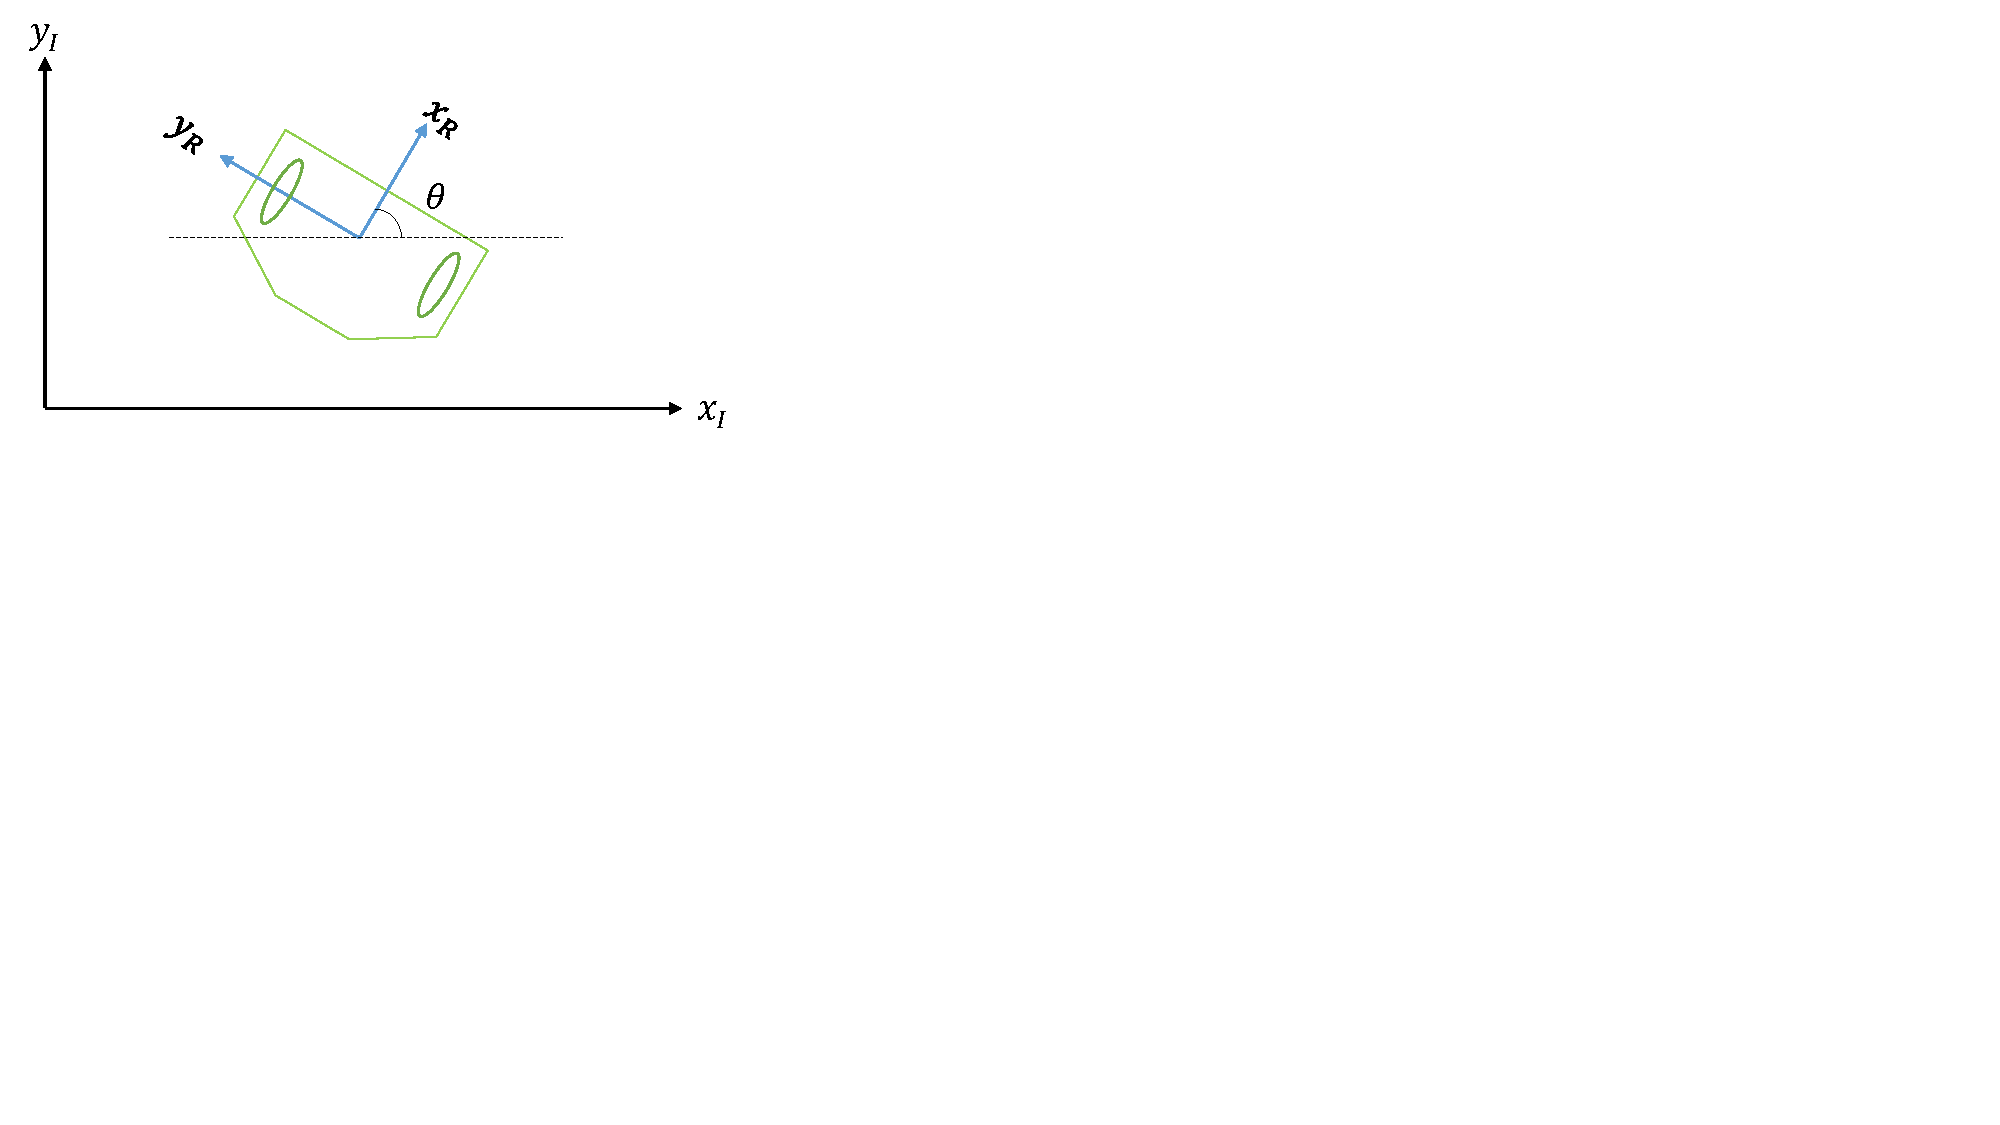
\includegraphics[clip,trim=0 11cm 21.5cm 0  ,width=0.5\linewidth]{./robotdiagram.pdf}
\caption{Inertial and robot frames of reference}
\label{fig:robotdiagram}
\end{figure}

\begin{equation}
X_I = 
	\begin{bmatrix}
	\cos\theta & -\sin\theta & 0 \\
	\sin\theta & \cos\theta & 0 \\
	0 & 0 & 1
	\end{bmatrix} X_R \label{rotation}
\end{equation}

The state vector of the system is $X = \left[x_I,y_I,\theta,\phi_R,\phi_L,\xd_I,\yd_I,\thetad,\dot{\phi}_R,\dot{\phi}_L\right]^T$ where $\phi_x,\dot{\phi}_x$ are the angle and angular velocity of the left and right wheel. The subscript 'I' is dropped for the inertial frame position and linear velocity. The control vector of the system is $U = [\tau_R,\tau_L]^T$ where $\tau_x$ is the torque applied to the left and right wheel. The coordinates are also represented as $q = [x_I,y_I,\theta,\phi_R,\phi_L]$ for ease.

The dynamic constraints on the system are determined by using the following assumptions:
\begin{enumerate}
\item The centre of mass is at the centre of symmetry ($y_R$ axis) and along the axis of applied torque at the wheels ($y_R$ axis)
\item No skidding of the wheels: $yd_R = 0 $
\item No slipping of the wheels
\end{enumerate}
The angular velocity of the robot $\thetad$ is related to the angular velocity of the wheels by Figure \ref{fig:robotschematic}.  
\begin{figure}
\centering
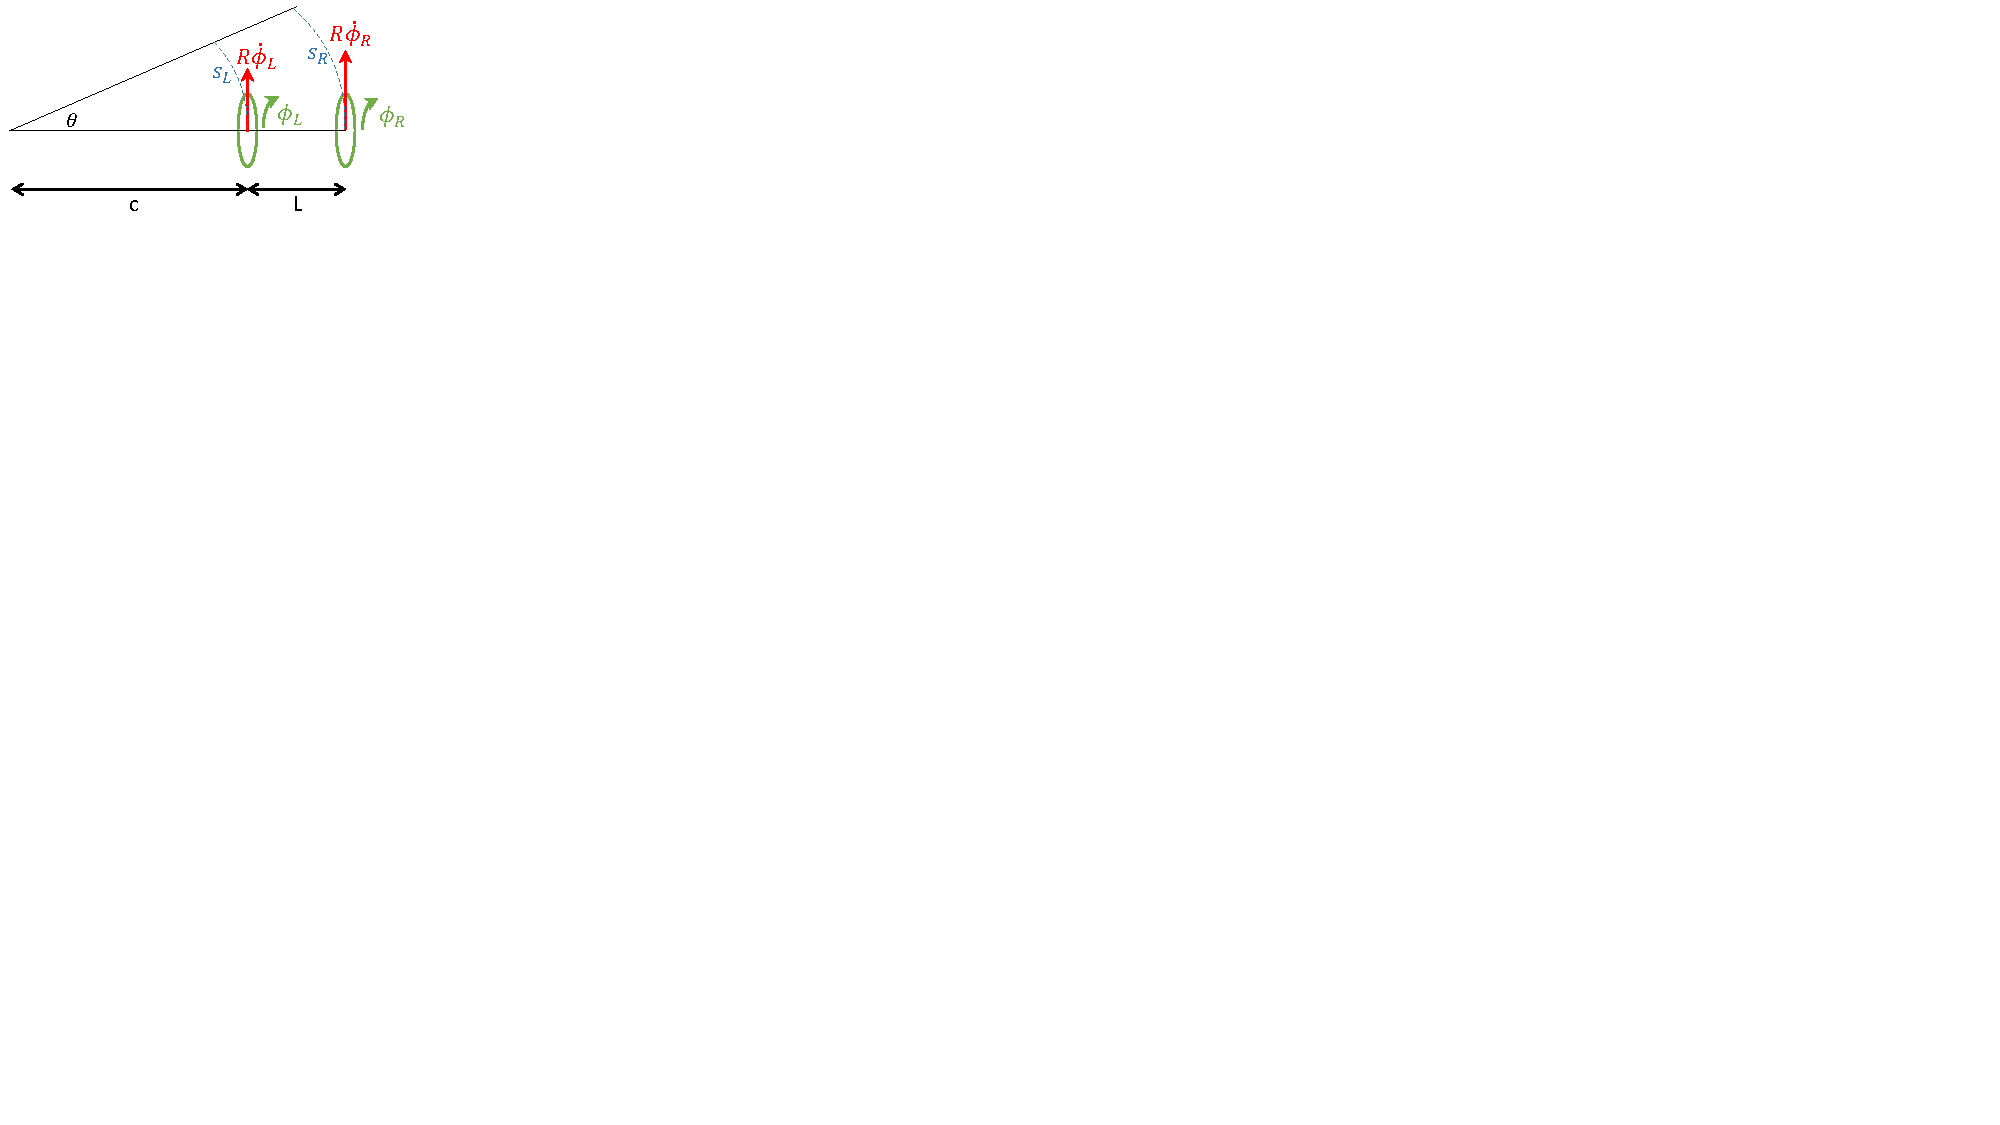
\includegraphics[clip,trim=0 15cm 27cm 0, width=0.5\linewidth]{./robotschematic}
\caption{Diagram of the differential drive of the robot. Where R is the radius of the wheels.}
\label{fig:robotschematic}
\end{figure}

\begin{eqnarray}
s_L &=& c\theta \nonumber\\
\frac{ds_L}{dt} &=& c\frac{d\theta}{dt} \nonumber\\ 
R\dot{\phi}_L &=& c\thetad \label{langles}\\
s_R &=& (c+L)\theta \nonumber\\
\frac{ds_R}{dt} &=& (c+L)\frac{d\theta}{dt} \nonumber\\ 
R\dot{\phi}_L &=& (c+L)\thetad \label{rangles}
\end{eqnarray}
As $\thetad$ must be equal for both Eq. \eqref{langles} \eqref{rangles}, the radius of curvature c is Eq. \eqref{radc}. This results in Eq.\eqref{eqthetad} for the no skid constraint.
\begin{eqnarray}
\frac{R\dot{\phi}_R}{R\dot{\phi}_R} &=& \frac{c+L}{c}\nonumber\\
c &=& \frac{L\dot{\phi}_L}{\dot{\phi}_R - \dot{\phi}_L} \label{radc}\\
\thetad &=& \frac{R}{L}\left( \dot{\phi}_R - \dot{\phi}_L \right) \label{eqthetad}
\end{eqnarray}
The inertial velocity of the robot is the average linear velocity of each wheel. This results in the relationship between the inertial states and the wheel states:
\begin{equation}
\begin{bmatrix}
\xd \\ \yd \\ \thetad
\end{bmatrix} = 
\begin{bmatrix}
\frac{R}{2}\left( \dot{\phi}_R + \dot{\phi}_L \right)\cos\theta \\
\frac{R}{2}\left( \dot{\phi}_R + \dot{\phi}_L \right)\sin\theta \\
\frac{R}{L}\left( \dot{\phi}_R - \dot{\phi}_L \right) 
\end{bmatrix} \label{cons}
\end{equation}
The constraint matrix C(q) is defined as $C(q)^T\dot{q} = 0$. Rearranging Eq.\eqref{cons} into this form is:
\begin{equation}
C(q) = \begin{bmatrix}
\cos\theta & \sin\theta & 0 & -R/2 & -R/2 \\
-\sin\theta & \cos\theta & 0 & 0  & 0\\
0 & 0 & 1 & -R/2 & R/2
\end{bmatrix}
\end{equation}


\paragraph{Dynamics of a Differential Drive Robot}
Lagrangian dynamics of the system are governed by the euler-lagrange equation for each coordinate:
\begin{eqnarray}
\frac{d}{dt}\left( \frac{\partial \Lagr}{\partial \dot{q}_i} \right)+\frac{\partial \Lagr}{\partial q_i} = F + C(q)^T\lam \label{ELE}
\end{eqnarray}
Where $\lam = [\lambda_1,\lambda_2,\lambda_3]^T$ are the Lagrangian multipliers associated with the constraints. F is the force vector defined as $[0,0,0,\tau_R,\tau_L]$. $\Lagr$ is the Lagrangian Eq.\ref{lag}, which is defined by the difference between the kinetic and potential energy of the system.
\begin{eqnarray}
\Lagr = \mathcal{T}-\mathcal{V} \label{lag}
\end{eqnarray}
The kinetic energy $\mathcal{T}$ of the robot is the sum of the translational and rotational kinetic energy of the body and each wheel. There is no potential energy as the robot is only used in the x-y plane. \textbf{velocity of each wheel}
%\begin{eqnarray}
%\Lagr &=&  \frac{1}{2}m_t\left( \xd^2+\yd^2 \right) + \frac{1}{2}I_t\thetad^2+\frac{1}{2}I_w\left( \dot{\phi}_R^2 + \dot{\phi}_L^2\right)+\frac{1}{2}\left( v_{w_L}^2 +v_{w_R}^2\right)
%\end{eqnarray}
%Where $v_{w_L}$ and $v_{w_R}$ are the linear velocities 
\begin{eqnarray}
\Lagr &=& \frac{1}{2}m_t\left( \xd^2+\yd^2 \right) + \frac{1}{2}I_t\thetad^2+\frac{1}{2}I_w\left( \dot{\phi}_R^2 + \dot{\phi}_L^2\right)
\end{eqnarray}
The equations of motion are then calculated from Eq.\eqref{ELE} and stored in the form Eq.\ref{form}. Where M(q) is a diagonal matrix with elements $[m_t,m_t,I_t,I_w,I_w]$. Which can be rearranged to calculate the acceleration of coordinates to be used for integration.
\begin{eqnarray}
M\ddot{q}-C(q)^T\lam &=& F \label{form}\\
\ddot{q} &=& M^{-1}[F+C(q)^T\lam] \label{qdd}
\end{eqnarray}
To solve for $\lam$, the time derivative of the constraints must equal zero as the constraints are constant.
\begin{eqnarray}
\frac{d}{dt}\left( C(q)\dot{q}\right) = 0\\
C(q)\ddot{q}+\dot{C}(q)\dot{q} = 0 \label{dc}
\end{eqnarray}
Substituting in \eqref{qdd} into \ref{dc}:
\begin{eqnarray}
CM^{-1}(F+C^T\lam)+\dot{C}\dot{q} &=& 0
\end{eqnarray}
Which results in
\begin{eqnarray}
\lam &=&-\left( CM^{-1}C^T \right)^{-1}\left( CM^{-1}F+\dot{C}\dot{q} \right)
\end{eqnarray}
The total time derivative of the constraint matrix is
 \begin{equation}
 \dot{C}(q) = \begin{bmatrix}
 -\thetad\sin\theta & \thetad\cos\theta & 0 & 0 & 0 \\
 -\thetad\cos\theta & -\thetad\sin\theta & 0 & 0 & 0\\
 0 & 0 & 0 & 0 & 0
 \end{bmatrix}
 \end{equation}
Using matlab symbols $\lam$ is solved as
\begin{equation}
\lam = \begin{bmatrix}
\frac{m_tR(\tau_L+\tau_R)}{R^2m_t+2I_w} - \frac{\thetad\left( \yd\cost-\xd\sint \right)}{R^2m_t+2I_w} \\
m_t\thetad \left( \xd\cost+\yd\sint \right)\\
\frac{I_tLR}{I_wL^2+2I_tR^2} (\tau_R-\tau_L)
\end{bmatrix}
\end{equation}
The lagrange multipliers are substituted into Eq.\eqref{qdd}, then the time derivative of the state vector is $\dot{X}=[\dot{q},\ddot{q}]^T$.

\paragraph{Optimisation}
 The cost function is applied over the time horizon T with accumulating least squares cost l(X,U) and final cost $V_T(X)$.
 \begin{eqnarray}
 J &=& \sum_{t = 0}^{T-1}  l(X,U)  + V_T(X)\\
 J &=& \sum_{t = 0}^{T-1} \left( (X-X_{ref})Q(X-X_{ref})+U(t)RU(t) \right) + (X_T-X_{ref})Q(X_T-X_{ref})
 \end{eqnarray}
 It is this cost function that is to be minimised in order to find the optimal set of control inputs. Using Pontryagin's Maximum Principle the hamiltonian in Eq.\eqref{hamil}, the 'direction' in state space for the minimum cost is calculated. This is because in state space the total cost is approximated as a quadratic function and has a global minimum (convex optimisation). 
 \begin{eqnarray}
 H(X,\Lambda,U) = l(X,U)+\Lambda^T(t)\dot{X}(X,U) \label{hamil}
 \end{eqnarray}
  Where $\Lambda$ is the adjoint trajectory with a boundary value at time T, it is then integrated backwards in time using runge kutta to find the adjoint trajectory at each timestep.
 \begin{eqnarray}
 \Lambda(T) &=& \frac{\partial V}{\partial X}\\
 \dot{\Lambda}(t) &=& -\frac{\partial H}{\partial X}
 \end{eqnarray}
 The search direction for the optimal control inputs is then Eq.\eqref{search} with the corresponding $\Lambda$.
 \begin{eqnarray}
 s(t) = -\frac{\partial H}{\partial X} \label{search}
 \end{eqnarray}
 
%\begin{eqnarray}
%\ddot{x} = -\thetad \left( \xd \cost\sint + \yd\sin^2(\theta)  \right) - 2I_w\thetad\left( -\xd \sint\cost + \yd \cos^2(\theta) \right) +   \label{xdd}
%\end{eqnarray}






\end{document}